\chapter{Ansatz}\label{ansatz}
Nachdem die Problemstellung geklärt ist und die konkurrierenden Technologien erläutert wurden, sollen nun die zugrundeliegenden Gedanken zur Problemlösung behandelt werden.
\section{Objektstruktur}
Zunächst würden die entsprechenden Modundellklassen aus der Xtext Grammatik in Scala Quellcode übernommen werden müssen. Style-, Shape-, Connection- und Diagramklassen mit entsprechenden Feldern würden zunächst als sogenannte \textit{case classes} erstellt werden. Dies würde den Vorteil haben im Falle einer später notwendigen verifizierung der Instanzen vorimplementierte hash- equals- und toString Methoden zur Verfügung zu haben. Da Style am flexibelsten ist (nur eingehende Abhängigkeiten) würde Style.scala zuerst erstellt werden und entsprechend der Assoziationsreihenfolge dann Shape.scala und Diagram.scala. \ref{diagramshapestyle}.
\subsection{ClassHierarchy}Da es für die Instanzen mancher Modellklassen möglich sein soll, Objekte der selben Klasse zu erweitern, war die Idee des Authors, eine Collection namens \textit{ClassHierarchy} zu erstellen, welche in der Lage sein sollte, ähnlich eines Baumes Vererbungshierarchien in Form von Knoten (\textit{Nodes}) darzustellen  \ref{classhierarchy}. So würden die Modellklassen, für die die Vererbung möglich sein soll, über diesen Baum in Relation gesetzt werden können. Im Falle einer gänzlich neuen Modellklasse (z.B. ein neuer Style) würde die Instanz als neue Basisklasse eingefügt werden, ansonsten über eine Methode, die beispielsweise \textit{inheritsFrom} heißen könnte. \textit{InheritsFrom} müsste entweder von der ClassHierarchy oder den Nodes selber zur Verfügung gestellt werden und würde über seine Argumente vermittelt bekommen, welche Knoten erweitert werden. \textit{InheritsFrom} würde dann eigenständig die \textit{parent}- und \textit{children} Listen eines Knotens um die neue Instanz der Modellklasse ergänzen.
\begin{figure}[H]
\begin{center}
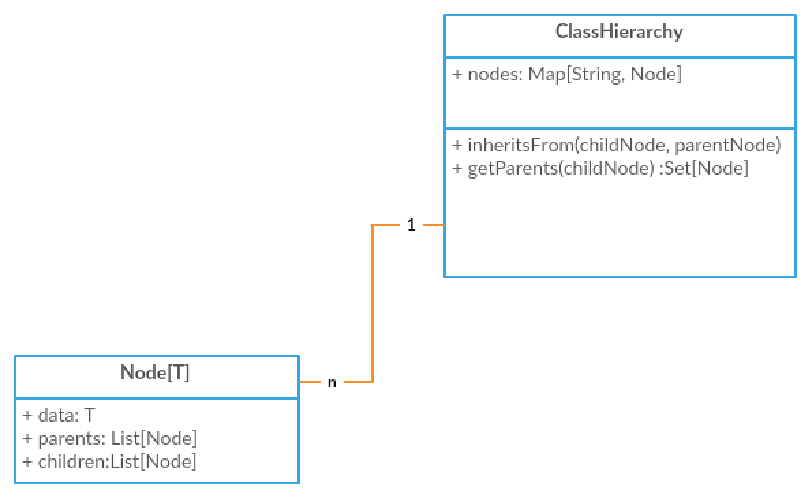
\includegraphics[scale = 0.7]{Bilder/classhierarchy.pdf}
\caption{Klassenmodell von ClassHierarchy}
\label{classhierarchy}
\end{center}
\end{figure}Wie in \ref{classhierarchy} zu sehen ist würden die Nodes über Listen verfügen, welche auf Elternknoten und auf Kindknoten verweisen. So könnte man bequem von jedem Style erfahren, welche Styles er erweitert und welche Styles ihn erweitern. Außerdem würde ClassHierarchy eine Map enthalten, welche Namen(strings) auf beliebige Klassen abbilden kann. Über dieses mapping wäre ein schneller Zugriff auf die gewünschte Klasse möglich, ohne mühsam durch eine Baumstruktur der Nodes navigieren zu müssen.
Um dieses Prinzip auf alle möglichen Klassen anwenden zu können sollte ClassHierarchy generisch sein. Vorausgehend waren die Anforderungen für Vererbung nur auf Style bezogen, da die Vererbungsprinzipien aber auch bei Shape hilfreich sein könnten, wäre so gewährleistet, dass man sich diese Tür nicht unnötig verschließt. 
Benötigte Enumerationen und andere nicht komplexe Hilfsobjekte der Klassen würden in dessen \textit{Companionobject} definiert werden. 
Über entsprechende Apply-Methoden sollte der Aufruf der ClassHierarchy so einfach wie möglich gestaltet werden. Um Aufrufe wie
\begin{lstlisting}[style=scala, aboveskip=0pt]
classHierarchy.nodes.get("styleName").data
\end{lstlisting}
zu vermeiden, würde eine apply-Methode benutzt werden um den Aufruf auf:
\begin{lstlisting}[style=scala, aboveskip=0pt]
classHierarchy("styleName")
\end{lstlisting}
zu verkürzen. Da der Aufruf in diesem Fall sehr eindeutig ist, kann ruhigen Gewissens auf die apply-Methode zurückgegriffen werden. \citet[p. 76 Fazit]{esser:scala}

\section{Parser}Neben den Gedanken zur Vererbung der Modellklassen, ist es auch wichtig zu klären, wie die Modelle überhaupt aus der Stringform in Objektform umzuwandeln sind. Entsprechende Mechanismen werden allgemein als Parser bezeichnet. Dieser Parser ist verantwortlich dafür die in Stringform enthaltenen Styles, Shapes, Connections und Diagrams als diese zu identifizieren und in Objekte umzuwandeln. 
Die Struktur eines Styles (ähnlich auch bei den anderen Modellen) ist in Listing \ref{lst:beispielstyle} beispielhaft dargestellt.
\begin{center}
\label{lst:beispielstyle}
\begin{lstlisting}[style=spray, caption={Beispielhafte Style Definition über die entsprechende Style DSL},label={lst:beispielstyle}]
style BpmnDefaultStyle {

	description = "The default style of the petrinet diagram type."
	
	transparency = 0.95

	background-color = black
	
	line-color = black

	line-width = 1

	font-color = black

	font-name = "Tahoma"
	
	font-size = 6

	font-bold = yes

	font-italic = yeshttp://www.macwrench.de/wiki/Kurztipp_-_Quellcodelistings_in_LaTeX

	gradient-orientation = horizontal
	und
}
\end{lstlisting}
\end{center}
Shapes und Diagrams fangen entsprechend mit
\begin{lstlisting}[style=spray, aboveskip=0pt]
shape/diagram <shapeName> {
\end{lstlisting} an.
Die Xtext Grammatik sollte außerdem um die Vererbungskomponente erweitert werden können, z.B.:
\begin{lstlisting}[style=spray, aboveskip=0pt]
shape SomeShape extends StandardShape {
\end{lstlisting}Style erlaubt zwar bereits erweitert zu werden, doch was die Vererbung von Shapes und Mehrfachvererbung generell angeht besteht noch Bedarf, da Xtext nicht in der Lage ist, diese Features umzusetzen.
\subsection{Reguläre Ausdrücke}Da Stringevaluierung, wie vorangehend erörtert, nicht ergebnisführend war, soll im Folgenden ein weiterer Ansatz vorgestellt werden,
die \textit{Regulären Ausdrücke}. Über diese \textit{regulären Audrücke} könnte der Style gefiltert werden um so an an der Syntax der DSL vorbei zu kommen und an die eigentlichen Attribute zu gelangen.
Anhand des ersten Wortes soll der Parser erkennen, um welchen Modelltyp (Style, Shape, Diagram) es sich handelt. 
Weiter würde ein vordefiniertes Schlenter code hereüsselwört \textit{extends} eine zu erweiternde Instanz kennzeichnen.
Im Gegensatz zu diesen hartkodierten Schlüsselwörtern würden die restlichen Attribute wie
\begin{lstlisting}[style=spray, aboveskip=0pt]
line-width = 1
\end{lstlisting} einheitlich geparsed werden als
\begin{lstlisting}[style=spray, aboveskip=0pt]
attributeName = attributeValue
\end{lstlisting} und erst in einer tieferen Parserklasse oder dem entsprechenden Konstruktor aufgelöst werden. Auf diese Art und Weise würden wenige Regeln ausreichen um komplexe Ausdrücke abbilden zu können. So geparste Attribute bleiben zunächst in der Stringform. Ziel dieses Vorgehens ist es zunächst nur Attributsname und Attributswert zu ermitteln, sicherzustellen, dass Syntaxregeln eingehalten wurden und die Weitergabe eines einheitlichen Datentyps an tieferliegende Parserklassen.
Um die Strings zu parsen, werden \textit{reguläre Ausdrücke} verwendet.
Die wenig komplexen Styles sollten so einfach zu parsen sein. Shapes stellen den schwierigsten Teil beim Parsing dar, da geometrische Figuren(\textit{geometricModel}), wie Ellipsen oder Polygone ineinander geschachtelt werden können.
\subsection{Factory Klassen}
Es wird davon ausgegangen, dass Modellklassen durch Umwandlung aus einem bereitgestellten Stringinput erzeugt werden. Dieser Stringinput enthält alle notwendigen Informationen um eine einsatzfähige Instanz einer Modellklasse erzeugen zu können. Es ist wünschenswert die Erzeugung der Instanzen so konsistent wie möglich zu halten. Dies bedeutet möglichst wenige und klar definierte Wege eine Klasse zu erzeugen. Dies kann effektiv über eine sogenante \textit{Fabrik} (vgl. englisch \textit{Factory}) Klasse erreicht werden. Zur Erzeugung der Exemplare der Modellklassen wird so wenn möglich nur eine einzige Methode definiert, die schlussendlich auf den Konstruktor der Modellklasse verweist. Dies schließt allerdings noch nicht aus, dass Modellklassen auch anders erzeugt werden können. Scala stellt einen von Haus aus eingebauten Mechanismus zur Verfügung, die \textit{Companion Objects}. Scala hat sich von den in Java typischen statischen Variablen (Klassenvariablen) getrennt. Um das Prinzip der Objektorientierung konsequenter durchzusetzen stellt es hieirfür die Definition von Singleton Objekte zur Verfügung. Über das Schlüsselwort \textit{object} kann anstatt einer Klassen-, eine Objektdefinition erfolgen. Jegliche Felder eines solchen Objekts sind (in Java manier ausgedrückt) Instanzvariablen, jedoch importierbar. Allein die Möglichkeit auf diese Art und Weise Singleton Objekte zu erstellen deckt bereits eine Funktionalität der Fabrik Klassen ab. Wird ein solches Objekt in der selben Quelldatei wie eine Klassendefinition erstellt und haben Klasse und Objekt außerdem den gleichen Namen handelt es sich um \textit{Companion Object} und \textit{Companion Class}. Auf den ersten Blick sind \textit{Companion Objects} nur der Ansatz Klassenvariablen bereitzustellen und trotzdem dem objektorientierten Paradigma treu zu bleiben. Ein entscheidender Vorteil ist jedoch, dass so definierte Objekte auch auf die privaten Member der \textit{Companion Class} zugriff haben. Auf unseren Fall bezogen bietet sich also die Möglichkeit den Konstruktor der Modellklasse mit dem Schlüsselwort \textit{private} zu kennzeichnen. Folglich kann nurnoch das \textit{Companion Object} darauf zugreifen und wir können exklusiven Zugriff über eine Fabrik Methode des Companion Objekts anbieten. 
\subsection{Parserlogik}
Da in den bisherigen Gedanken geklärt worden ist, wie Strings eingelesen werden, die Vererbung unter den Modellklassen dargestellt werden kann und wie Modellklassen konkret erzeugt werden, kann nun anhand des Sequenzdiagramms \ref{sequenzdiagrammAnsatz} beschrieben werden wie ein Parsing Vorgang prinzipiell abzulaufen hat.\linebreak
\begin{figure}[htb]
	\hspace*{-0.5cm}
		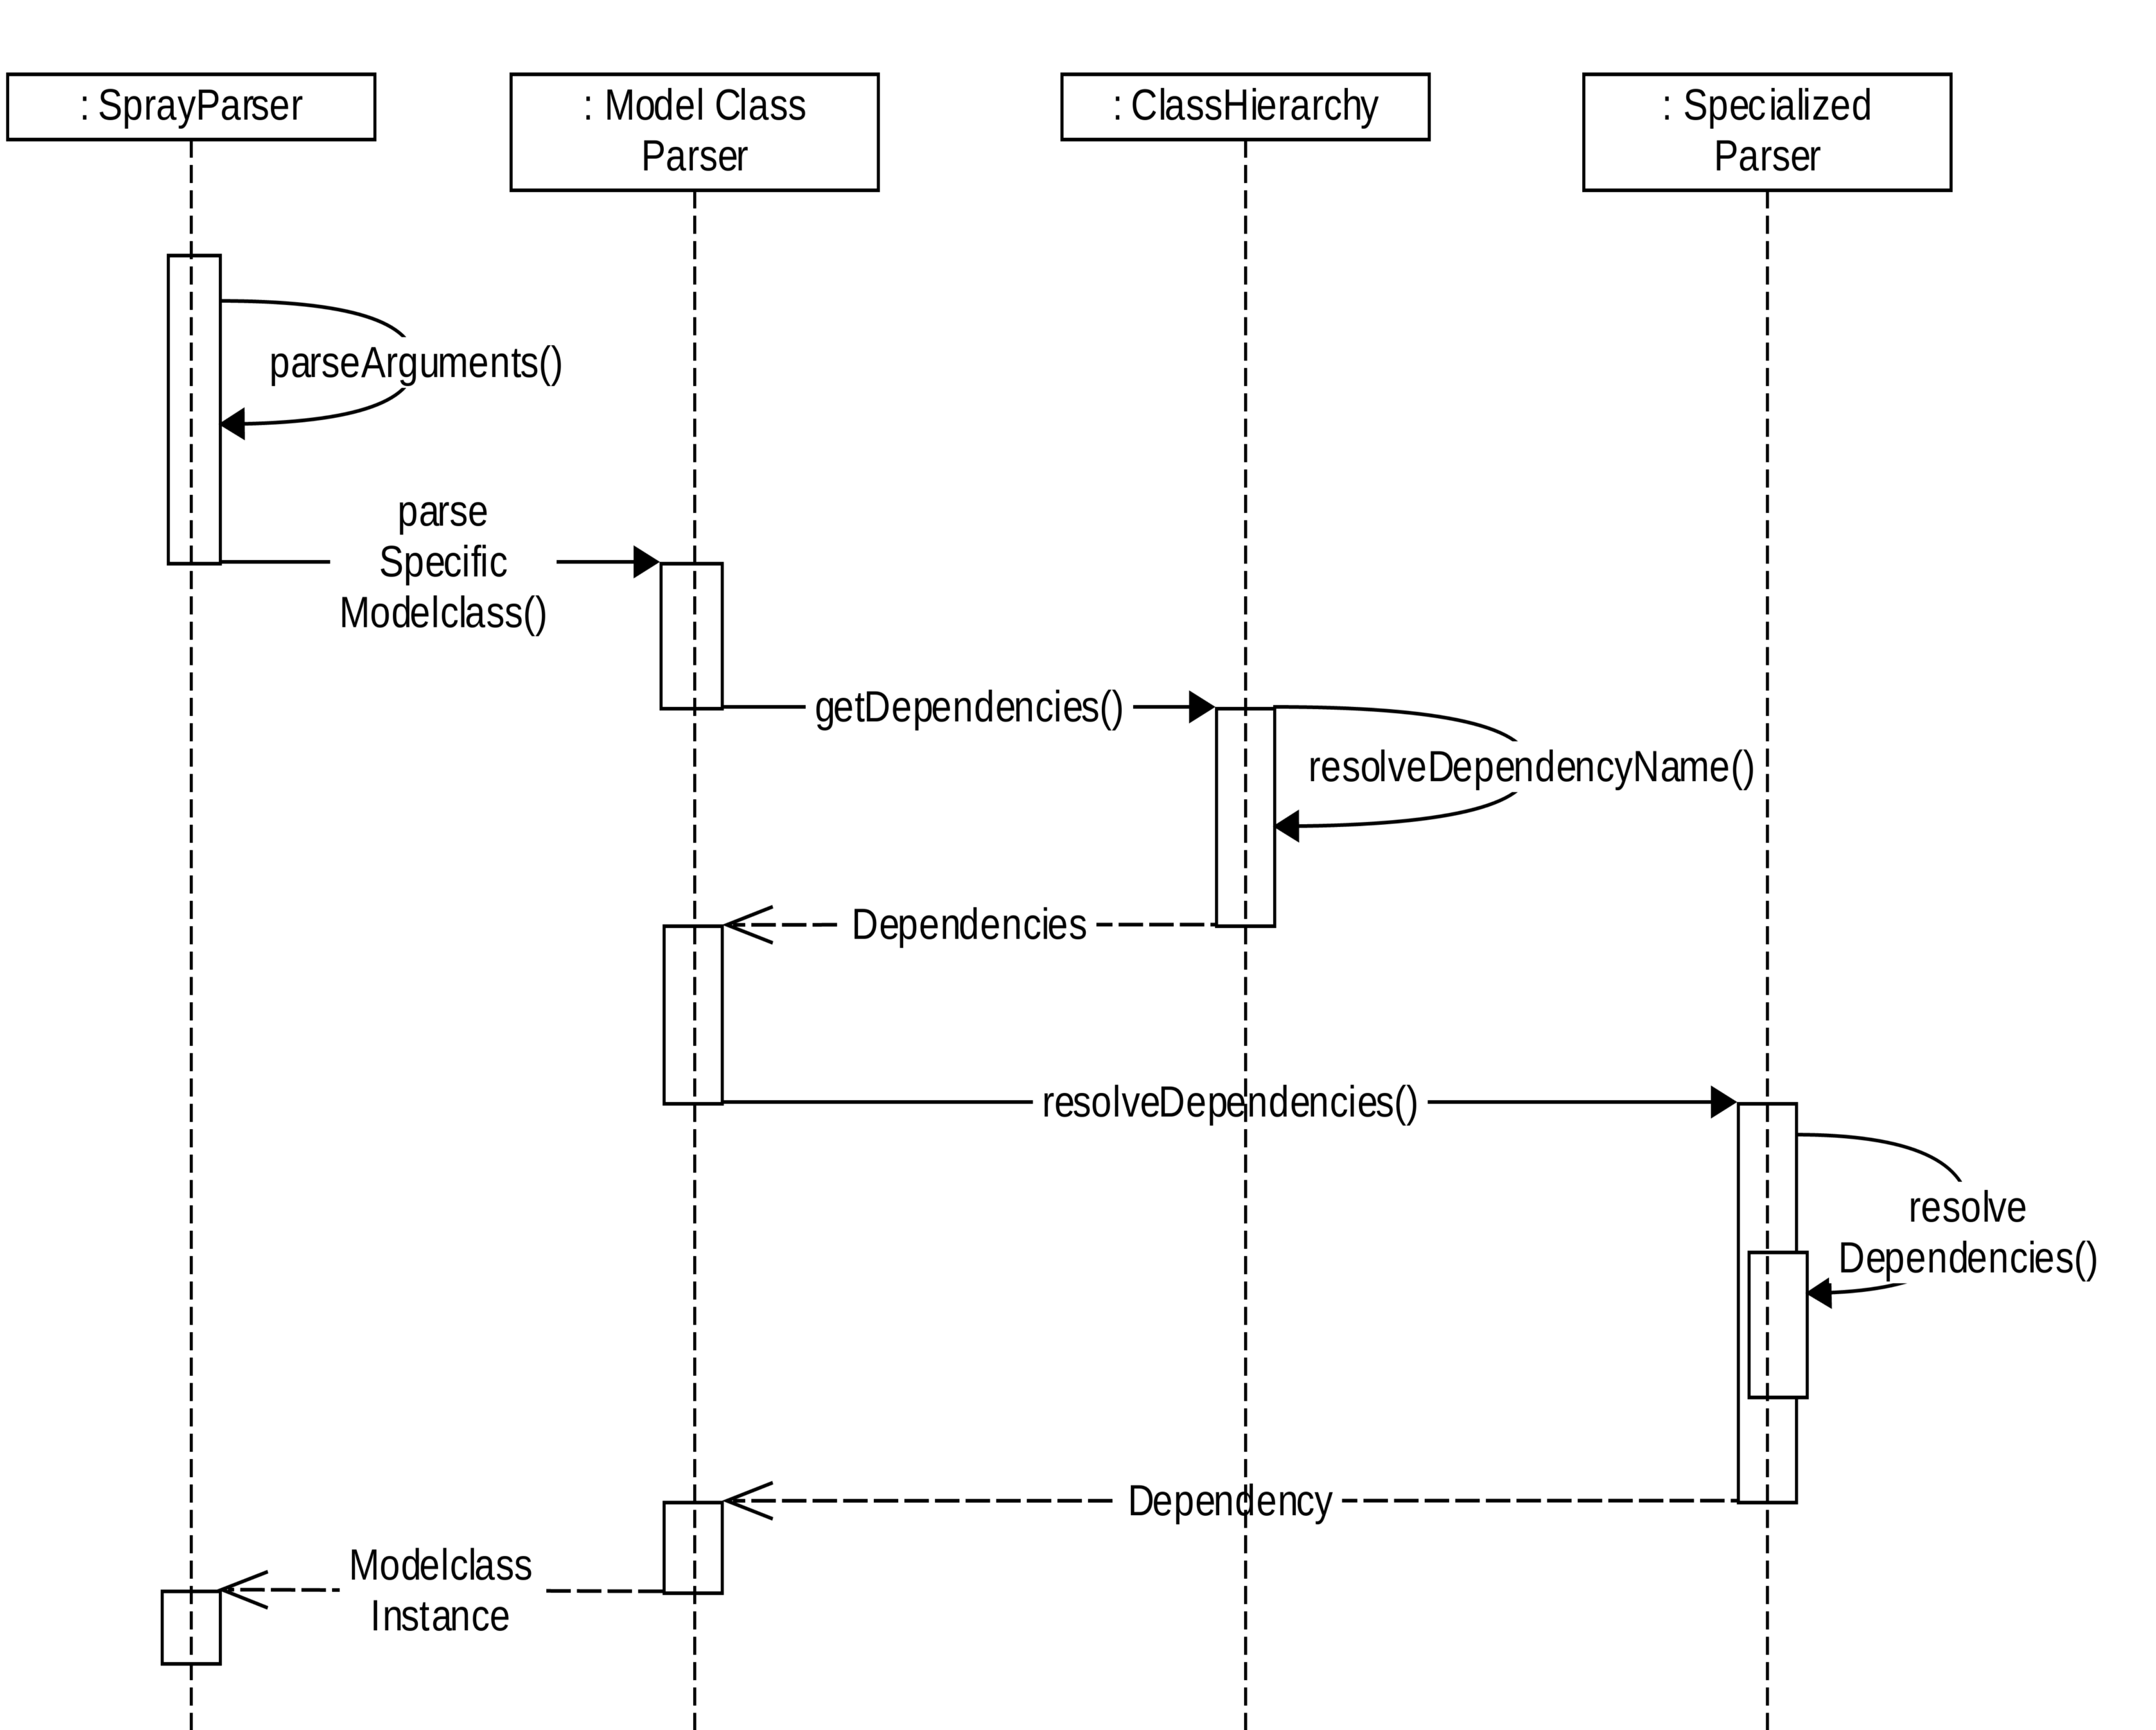
\includegraphics[scale = 0.13]{Bilder/sequenzdiagrammAnsatzKomprimiertScaled(2500x2500).png}
		\caption{Sequenzdiagramm für den Ablauf eines Parsing Vorgangs}
		\label{sequenzdiagrammAnsatz}
\end{figure}Erhält die Applikation einen String um beispielsweise eine Shape einzulesen, werden zunächst sämtliche Attribute aus dem String gefiltert. Hierzu zählen auch Name und erweiterte Shapereferenzen. Dies wird über eine Methode namens \textit{parseArguments}(vgl. \ref{sequenzdiagrammAnsatz}) erfolgen. Egal um welche Modellklasse es sich handelt, werden alle ausgelesenen Attribute in Stringform weiterverarbeitet. So wird die Verantwortung der Auflösung auf die einzelnen Parser der Modellklassen ausgelagert und diesen gleichzeitig ein einheitliches Medium geliefert. Auf diese Weise können ähnliche oder gleiche Attribute in unterschiedlichen Parsern auf die selbe Weise aufgelöst werden. Wie bereits angedeutet geht es von hier an mit einem auf die Modellklasse spezialisierten Parser weiter \textit{parseSpecificModelClass}(vgl. \ref{sequenzdiagrammAnsatz}). Der spezifische Modellklassenparser muss nun zunächst prüfen, ob weitere Instanzen, des Zieltyps erweitert werden sollen. Hierfür gibt er die in den Attributen enthaltene Liste an Eltern (in Form von Strings) an die \textit{ClassHierarchy} weiter, die den Überblick über die Vererbungshierarchie hat und die Namen über ein internes Mapping auf bestehende Referenzen auflösen kann (\textit{resolveDependencyName}, vgl. \ref{sequenzdiagrammAnsatz}). Sind alle Elternteile aufgelöst, kann der Modellklassen spezifische Parser nun anhand einer kompletten Liste an Attributen beginnen die in Stringform enthaltenen Informationen der Abhängigkeiten aufzulösen.
Falls es sich bei den in Stringform enthaltenen Informationen nicht um primitive Datentypen, sondern um komplexe evtl. ineinander geschachtelte Elemente handelt, werden diese wiederum an ihren speziell definierten Parser weitergegeben (\textit{resolveDependencies}, vgl. \ref{sequenzdiagrammAnsatz}). Da die Elemente wie gesagt evtl ineinander verschachtelt sind, können viele weitere rekursive Aufrufe auf spezialisierte Parsereinheiten erfolgen, bis schließlich alle Argumente aufgelöst sind und eine fertige Instanz an den SprayParser zurück geliefert werden kann. Die Parserlogik teilt sich also auf viele kleine spezialiserte Parser auf. Dabei gibt es einerseits den SprayParser, welcher die Schnittstelle zu allen vorhandenen Parsern darstellt, die vier spezialisierten Style-, Shape-, Connection- und Diagramparser, welche die Modellklassen erzeugen und einige weitere kleinere Parser, welche dafür verantwortlich sind eigens erstellte Datentypen parsen und erzeugen zu können, wie zum Beispiel \textit{Anchor}s. 
\section{Auflösung von Vererbungshierarchien}
Ist eine Technik gefunden, mit der sich die DSL in die Objektstruktur der Modellklassen umwandeln lässt, muss direkt die Problematik der Vererbung betrachtet werden, da die hierfür benötigten Techniken schon beim Parsen beachtet werden müssen. Es soll ein Vererbungsmechanismus implementiert werden. Entgegen der geläufigen Definition der Vererbung handelt es sich hierbei nicht um das Erweitern von Klassen, wie man es aus diversen Programmiersprachen kennt. Die Anforderung definiert, dass einzelne Instanzen der Modellklassen in der Lage sein sollen Objekte der selben Klasse erweitern zu können. Genauer bedeutet dies, dass eine Instanz \textbf{nicht} in der Lage sein soll dynamisch komplett neue Attribute zu definieren, sondern \textbf{bekannte} Attribute von Elterninstanzen zu übernehmen, beziehungsweise zu überschreiben. Erweitern soll in diesem Kontext also zwei Situationen beschreiben:
\begin{itemize}
\item Elternteil verfügt über Attribute, die in der erweiternden Klasse nicht vorhanden sind -\textgreater Wert wird geerbt
\item Elternteil verfügt über Attribute, die in der erweiternden Klasse vorhanden sind -\textgreater ignoriere/überschreibe den Wert der erweiterten Klasse
\end{itemize}
Das folgende Beispiel, soll verdeutlichen was gemeint ist:
Es wird eine vereinfachte Styleklasse definiert
\begin{lstlisting}[style=scala]
class Style(val name:String, val transparency:Double, val line-width:Int)
\end{lstlisting}Nun wird eine Instanz (S1) der Modellklasse über die DSL definiert, welche sowohl einen Namen, als auch eine Angabe zur \textit{transparency} hat:
\begin{lstlisting}[style=spray]
style S1 {
    transparency = 0.5
}
\end{lstlisting}Eine weitere Instanz (S2) wird definiert, die ihrerseits über einen Namen und eine Angabe zur \textit{line-width} verfügt. Außerdem soll S2 die Instanz S1 erweitern:
\begin{lstlisting}[style=spray]
style S2 extends S1{
    line-width = 10
}
\end{lstlisting}
Nach diesen Definitionen sollten Objekte folgender Struktur entstanden sein (aus Gründen der Lesbarkeit aufgeführt in der Java Script Object Notation):
\begin{lstlisting}[style=spray]
{
 "name": "S1",
 "transparency": 0.5,
 "line-width":"notDefined"
}

{
 "name": "S2",
 "transparency": 0.5,
 "line-width": 10
}
\end{lstlisting}Wie man sieht verfügt S2 über eine \textit{transparency} angabe, die von S1 übernommen wurde. Wenn an dieser Stelle jedoch Überlegungen zur Implementierung unternommen werden, wird man mit folgenden Fragen konfrontiert:
\begin{itemize}
\item Wie weiß ein Objekt, dass es das Attribut des Elternteils übernehmen oder überschreiben soll?
\item Übernimmt S2 tatsächlich alle Attribute des Elternteils, oder hält es nur eine Referenz auf S1?
\end{itemize}Die meisten der Attribute, die in der Definition einer Modellklasse berücksichtigt werden können, sind optional. Wie man bei der Definition von S1 sieht, wurde keine Angabe zur \textit{line-width} gemacht. Da die Definition jedoch auf den Konstruktor der Style Klasse abgebildet wird, muss irgendwo eine konkrete Angabe zu dem \textit{line-width} Attribut erfolgen. Man könnte sich überlegen, jedem Feld der Modellklassen einen Defaultwert zuzuweisen. Das würde bedeuten, dass die \textit{line-width} beispielsweise standardmäßig auf 10 gesetzt wird, wenn in der Definition keine Angabe darüber gemacht wird. Hat aber folglich jede Styleinstanz zu jedem möglichen Attribut eine valide Angabe, fragt sich, woher später bekannt ist, ob auf Attribute einer Elterninstanz oder auf die eigenen zugegriffen wird. Immerhin gibt es zu jedem Feld der Instanz gültige Werte.
\subsection{Kennzeichnung nicht definierter Felder in Modellklassen}
Da Integerwerte ausschließlich gültige Werte haben wäre es sinnlos 0 als \textit{nicht gesetzt} zu verwenden und 1 - MAX\_INT als \textit{gesetzte Werte}. Am Beispiel der \textit{line-width} Angabe in S1 wird also klar, dass es bekannt sein muss, ob die Definition den Wert beschreibt, oder nicht. 
Deshalb werden alle Felder der Modellklassen (Style, Shape, Diagram), die ein konkretes Attribut der Modellklasse darstellen, als sogenannte \textit{Options} definiert. \textit{Options} sind dem Paradigma der funktionalen Programmierung zu verdanken(z.B. in Haskell -\textgreater Maybe).
Sie lösen ein Problem, welches in Java meist mit einer Exception gelöst wird.
Eine Funktion gibt nicht immer für jedes Argument ein gültiges Ergebnis zurück, \citet[p. 102]{esser:scala}. Im Falle der optional setzbaren Attribute der Modellklassen bieten Options daher die passende Lösung. Man kann sie entweder auf \textit{None} initialisieren oder auf ein \textit{Some$[$T$]$ }. Representativ steht also in diesem Fall \textit{None} für: nicht gesetzter Wert (schau in den Elternklassen nach entsprechenden Werten) und \textit{Some$[$T$]$} für: gesetzter Wert, ignoriere/überschreibe den Wert der Elternklasse.
\subsection{Vererbungsmechanismus über Referenz auf Elterninstanzen}
Als nächstes ist es derzeit auch noch unklar an welcher Stelle dieser Gedanke Anwendung findet. Es besteht einerseits die Möglichkeit erst beim unmittelbaren Zugriff auf die einzelnen Felder zu prüfen, ob sie definiert wurden, andererseits könnten jegliche Elterninstanzen schon bei der Erzeugung einer neuen Instanz nach fehlenden Werten durchsucht werden. Genauer ist also die Frage, ob Modellklassen eine zusätzliche Referenz auf Elternteile erhalten und nicht definierte Werte erst bei Bedarf in den Attributen der Elternliste gesucht werden, oder ob Modellklassen schon bei der Instanziierung über sämtliche Attribute der Eltern bescheid wissen, diese auf sich übertragen und anschließend nicht mehr auf ihre Eltern angewiesen sind. Beide Möglichkeiten bieten Vor- und Nachteile. Referenzen erlauben es, die Extraktionslogik der Attribute auf eine beliebige Stelle im Code auszulagern, je nach dem wann der Aufruf eben erfolgen soll. Außerdem erscheinen sie zunächst Speicherschonender. Die Überlegung wäre ja, dass nicht definierte Werte auch keinen zusätzlichen Speicher benötigen, somit kein zusätzlicher Speicher allokiert werden muss. Dies ist allerdings ein Trugschluss. Die Felder einer Styleinstanz werden immer initialisiert. Im Falle, dass der Wert in der Definition nicht angegeben wurde, eben mit besagtem \textit{None} Wert. Im Endeffekt ist also leiglich eine weitere Referenz als Attribut hinzugekommen, was die Speicherauslastung also (wenn auch unmerklich) erhöht.
\subsection{Vererbungsmechanismus durch direkte Weitergabe der Attribute bei Instanziierung}
Werden die Attribute der Elternklasse jedoch direkt bei der Objekterzeugung an die neue Instanz weitergegeben, hat dies zwei besondere Vorteile. Je nach Größe der Vererbungshierarchie ist es wesentlich performanter die Werte im aktuell benutzten Element zu suchen, als über eine Referenz in den vielen Elternknoten zu suchen. Außerdem beseitigt diese Vorgehensweise die Rekursivität der Problemstellung. Dazu ein stark vereinfachtes Beispiel:\linebreak Werden mehrere Modellklassen (hier Style) definiert, welche den jeweiligen Vorgänger erweitern und wird davon ausgegangen, dass die Attribute der zu erweiternden Instanzen direkt bei der Erzeugung übernommen werden,
\begin{lstlisting}[style=spray]
style S1 {}
style S2 extends S1 {}
style S3 extends S2 {}
style S4 extends S3 {}
\end{lstlisting}kann davon ausgegangen werden, dass S2 jedes Element von S1 erbt, S3 jedes Element von S2 erbt und somit auch implizit jedes Element von S1 usw. Diese Eigenschaft lässt sich auf beliebig viele erweiternde Instanzen anwenden, wodurch in dem Beispiel S4 garantiert jede Eigenschaft von S1, S2 und S3 enthält, oder überschreibt. Da die Rekursivität der Problemstellung so entfällt und den Code (ausschlaggebender Faktor ist die Größe des durch Vererbung erstellten Baumes) performanter gestaltet, wird versucht werden die Vererbungshierarchie auf diese Weise aufzulösen.

\section{Generatoren}Ausgehend davon, dass nun Strings eingelesen und in entsprechende Instanzen der Modellklassen umgewandelt werden können, ist der nächste Schritt über Generatoren den nun eigentlich gewünschten Code (Generat) erzeugen zu lassen. Hierfür gibt es entsprechend der Modellklassen einige Generatorenklassen wie z.B. \textit{StyleGenerator}, welcher die Style Modellklassen abbildet oder auch den \textit{ShapeGenerator}, der die Shape Modellklassen abbildet. Die Generatorenklassen bilden die entstandenen Objektinstanzen auf \textit{javascript} code ab. Um der Vererbung entsprechend immer die richtigen (also evtl die überschriebenen) Werte zu bekommen, müssen stets erst die Eltern-Knoten besucht werden, um nachzusehen, ob ein Elternteil evtl einen Wert ausfüllt.

